\section{Reduction to Single Track model}
%
As highlighted in the previous section, the complete equations of motion are complex and cannot be shown. However, one way to validate the model is to reduce the problem to a simple case to observe the terms in the equation. As a proof of concept, one can isolate the two equation of motion of the whole motorcycle concerning the pitch and the vertical translation ($\theta$ and $h$).\\
%
%
From the equilibrium of momentum is clear that from those equation one can solve for the vertical forces. Those will have a complex formulation that simplified in the case of the motorcycle in vertical position ($\phi(t)=0$), no steering ($\delta(t)=0$), lateral velocity null ($v(t)=0$), zero yaw rate ($\Omega(t)=0$) and internal degrees of freedom frozen ($\eta(t)=\eta_{00}$, $\theta(t) = \theta_{00}$, $s_f(t)=s_{f_{00}}$). The equations are still complicated, but a lot of terms can be collected yielding the following expression.
%
\begin{equation}
    \label{eq:vertForces}
\begin{array}{c} 
\displaystyle
{\it Fzr} \left( t \right) =+{\frac {M_{{\it tot}}\,{\it ax} \left( t \right) {\it ZG}}{L}}+{\frac {{\it Ca}\,\left( u \left( t \right)  \right) ^{2}{\it ZA}}{L}}+{\frac {{\it Iy}_{{\it wf}}\,{\frac {{\rm d}^{2}}{{\rm d}{t}^{2}}}\theta_{f} \left( t \right) }{L}}+{\frac {{\it Iy}_{{\it wr}}\,{\frac {{\rm d}^{2}}{{\rm d}{t}^{2}}}\theta_{r} \left( t \right) }{L}}+{\frac {M_{{\it tot}}\,g{\it Lf}}{L}}\\
\displaystyle
{\it Fzf} \left( t \right) =-{\frac {M_{{\it tot}}\,{\it ax} \left( t \right) {\it ZG}}{L}}-{\frac {{\it Ca}\, \left( u \left( t \right)  \right) ^{2}{\it ZA}}{L}}-{\frac {{\it Iy}_{{\it wf}}\,{\frac {{\rm d}^{2}}{{\rm d}{t}^{2}}}\theta_{f} \left( t \right) }{L}}-{\frac {{\it Iy}_{{\it wr}}\,{\frac {{\rm d}^{2}}{{\rm d}{t}^{2}}}\theta_{r} \left( t \right) }{L}}+{\frac {M_{{\it tot}}\,g{\it Lr}}{L}}
\end{array}    
\end{equation}
%
In the previous equations $ax(t)$ is actually the longitudinal acceleration that in general is equal to $\frac {{\rm d}^{}}{{\rm d}{t}^{}}u(t)-\Omega(t) v(t)$. However, both $\omega(t)$ and $v(t)$ are considered null, therefore $\displaystyle ax(t) = \frac {{\rm d}^{}}{{\rm d}{t}^{}}u(t)$.
$L$ is the total length defined as $L= L_r+L_f$ where $L_r$ and $L_f$ are rear axis length and front axis length. Those are measure the distance of the contact point from the CoM of the motorcycle. $ZA$ is the height of the pressure point where the drag force is applied redefined in the reference frame $RF_1$.\\
The solution for the vertical forces in equation \ref{eq:vertForces} shows clearly the dependency on static load distribution between front and rear wheel due to the position of the centre of mass $\displaystyle{\frac {M_{{\it tot}}\,g{\it Lf}}{L}}$. The other therms depends on load transfer due to drag, to acceleration and wheels angular acceleration.\\
%
\begin{figure}[htb]
    \centering
    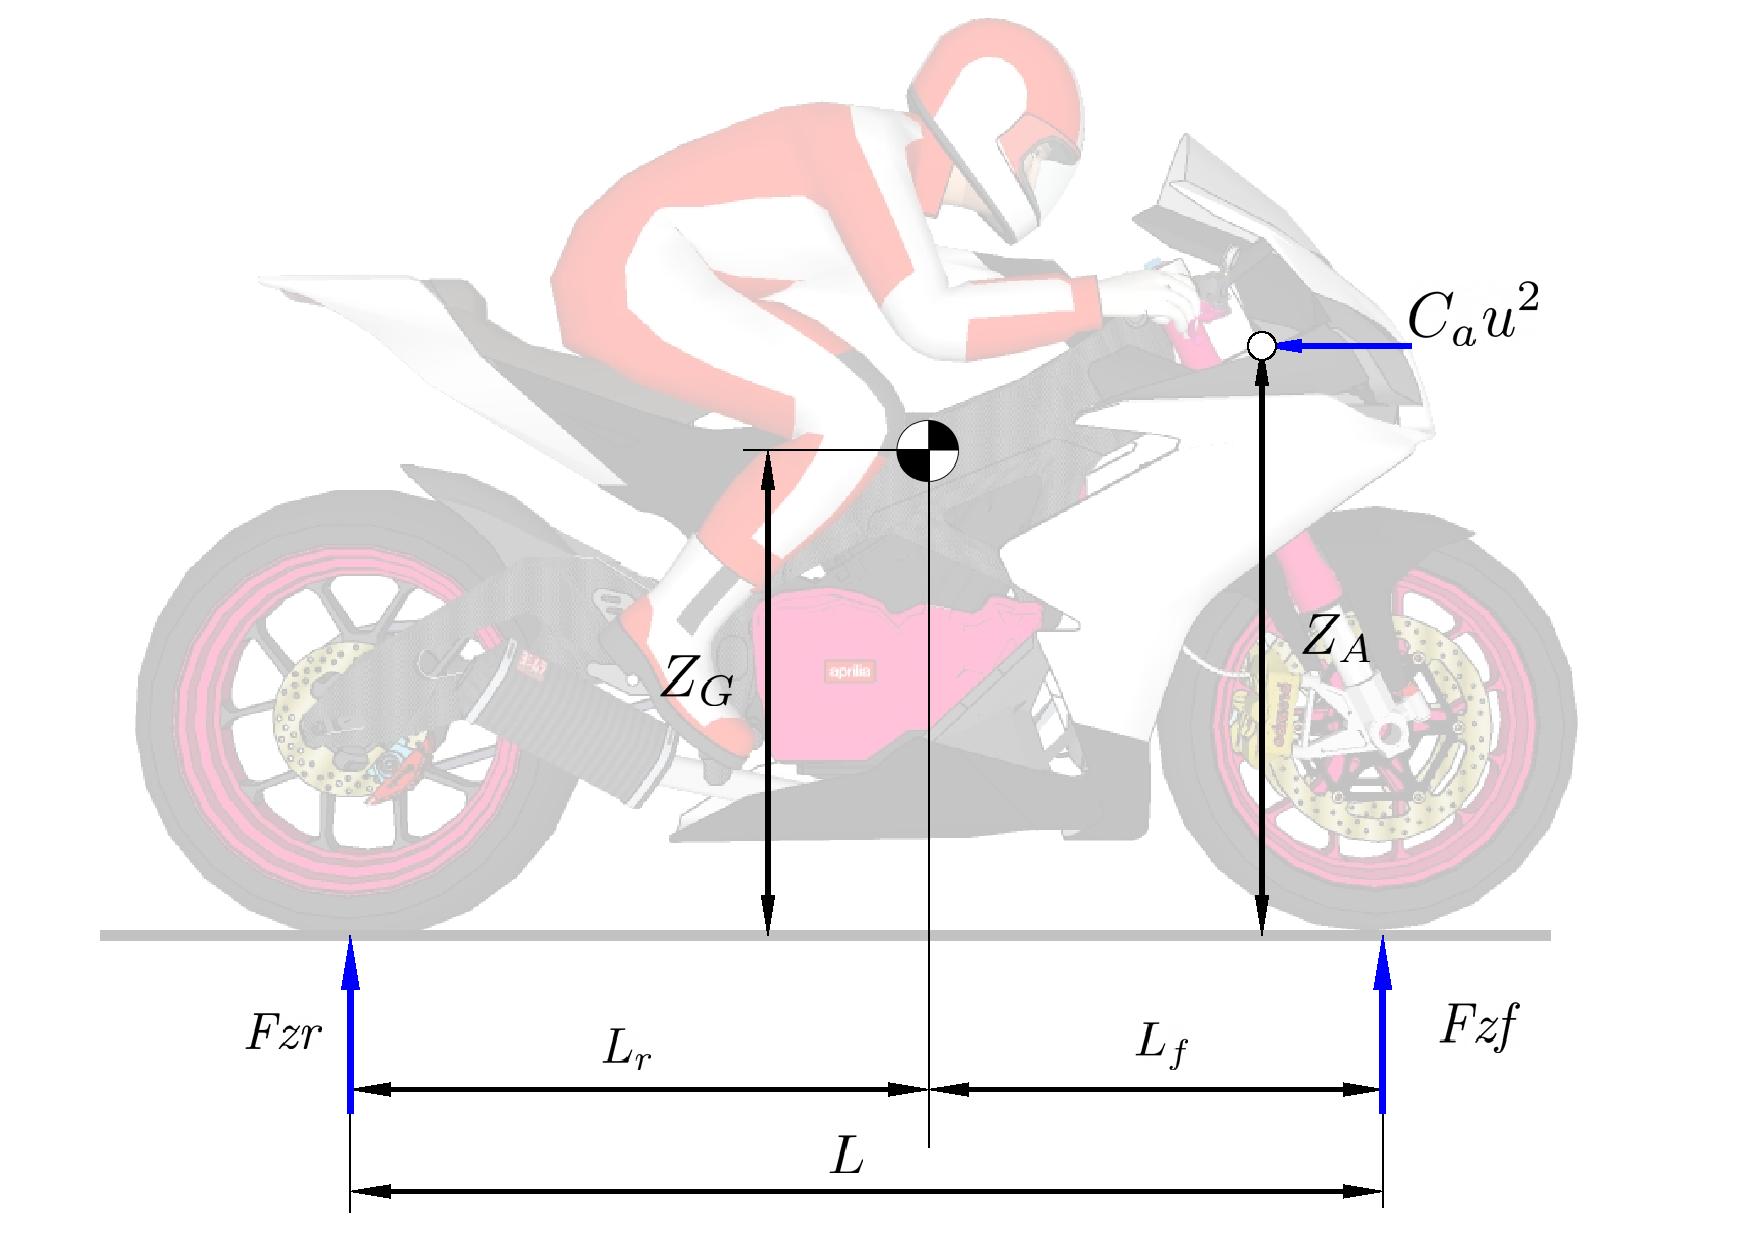
\includegraphics[width=\linewidth]{Coordinates/SingleTrackRed.pdf}
    \caption{Scheme of the single track reduction}
    \label{fig:SigngleTrackRed}
\end{figure}